\section{DICOM en pratique}

\frame
{
	\frametitle{Anonymisation}
	\begin{itemize}
		\item Utilisation d'images cliniques pour la recherche ou l'enseignement.
		\item Fichiers mis \`a disposition du public.
		\item N\'ecessit\'e d'anonymat : suppression des informations personnelles permettant d'identifier le patient.
		\begin{itemize}
			\item PatientsName (0010,0010)
			\item PatientID (0010,0020)
			\item PatientBirthDate (0010,0030)
			
			$\rightarrow$ de type 1 : \`a remplacer, pas supprimer !
			\item ReferringPhysicianName (0008,0090)
			\item etc.
			\item Potentiellement plus de 250 champs \`a supprimer ou \`a vider !
		\end{itemize}
	\end{itemize}
}

\frame
{
	\frametitle{DICOM Conformance Statement}
	\begin{itemize}
		\item Document pr\'ecisant le niveau de conformit\'e d'un produit (e.g. modalit\'e, logiciel, etc.) \`a la norme DICOM.
		\item Plan et structure pr\'ed\'efinis par la norme.
		\item Tr\`es technique :
		\begin{itemize}
			\item Diagrammes des flux de donn\'ees.
			\item Liste des services fournis.
			\item Liste des SOP Class support\'ees et des r\^oles assur\'es (SCU, SCP).
		\end{itemize}
		\item Exemple de DICOM Conformance Statement : OsiriX
		
		\url{https://www.osirix-viewer.com/pdf/DICOMConformanceStatements.pdf}
	\end{itemize}
}

\frame
{
	\frametitle{Achat d'un \'equipement}
	\begin{enumerate}
		\item Avant l'achat, soumission de l'appel d'offre :
		\begin{itemize}
			\item D\'efinition du sc\'enario de travail souhait\'e.

                Exemple : les images brutes export\'ees pourront \^etre r\'eutilis\'ees \emph{a posteriori}.
			\item R\'edaction du cahier des charges DICOM.
			\begin{itemize}
				\item Pr\'eciser le niveau d'exigence de DICOM.
				
				$\rightarrow$ faire appel \`a un consultant ou \`a des coll\`egues,
				
				$\rightarrow$ ou acqu\'erir le savoir-faire en interne.
				\item Demander le Document de Conformit\'e DICOM (DICOM Conformance Statement).
			\end{itemize}
		\end{itemize}
		\item Acceptation protocol\'ee.
		\begin{itemize}
			\item V\'erification de DICOM.
			\item V\'erification du/des sc\'enario/ii requis.
			\item Tests.
		\end{itemize}
	\end{enumerate}
}

\frame
{
	\frametitle{Services \`a demander}
	\begin{center}
		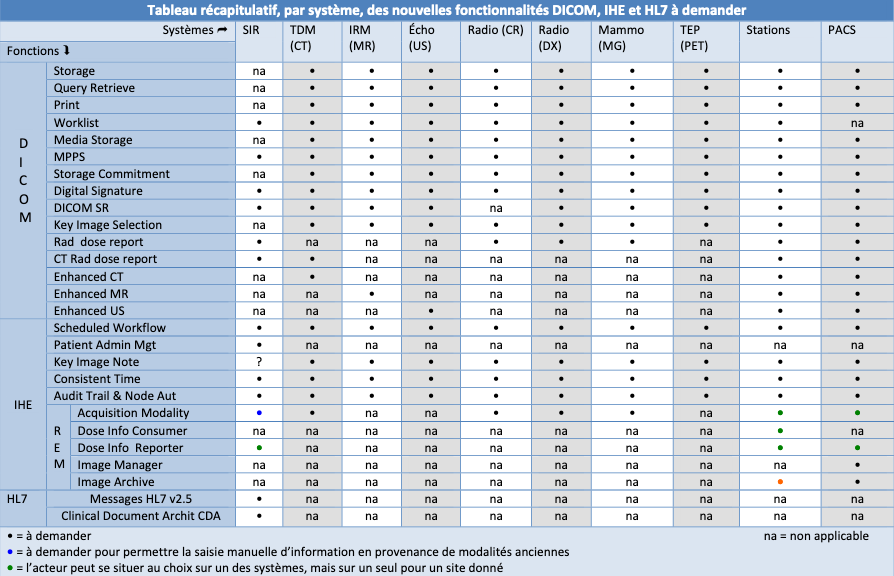
\includegraphics[width=\linewidth]{./figures/tableau-services.png}
	\end{center}
}

\frame
{
	\frametitle{\'Equipements non standards}
	
	\begin{itemize}
		\item Int\'egration possible dans un workflow DICOM via une passerelle de conversion.
		
		\begin{center}
			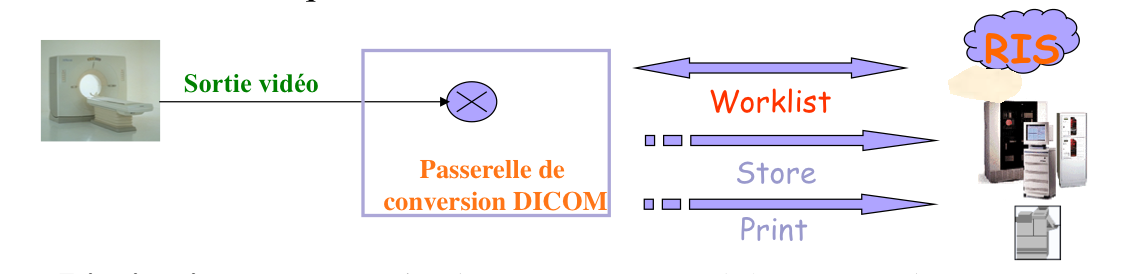
\includegraphics[width=\linewidth]{./figures/passerelle.png}
		\end{center}
		\item Limitation : images stock\'ees en mode Secondary Capture (IOD le plus simple de DICOM), les donn\'ees d'acquisition des images sont perdues.
	\end{itemize}
}

